\documentclass[12pt]{article}

\usepackage{graphicx}
\usepackage{paralist}
\usepackage{amsfonts}
\usepackage{amsmath}
\usepackage{hhline}
\usepackage{booktabs}
\usepackage{multirow}
\usepackage{multicol}
\usepackage{url}
\usepackage{hyperref}
\usepackage{graphicx}
\graphicspath{ {./images/} }

\oddsidemargin -5mm
\evensidemargin -10mm
\textwidth 170mm
\textheight 200mm
\renewcommand\baselinestretch{1.0}

\pagestyle {plain}
\pagenumbering{arabic}

\newcounter{stepnum}

%% Comments

\usepackage{color}

\newif\ifcomments\commentstrue

\ifcomments
\newcommand{\authornote}[3]{\textcolor{#1}{[#3 ---#2]}}
\newcommand{\todo}[1]{\textcolor{red}{[TODO: #1]}}
\else
\newcommand{\authornote}[3]{}
\newcommand{\todo}[1]{}
\fi

\newcommand{\wss}[1]{\authornote{blue}{SS}{#1}}

\title{Assignment 4, Design Specification}
\author{SFWR ENG 2AA4}

\begin {document}

\maketitle

\indent This Module Interface Specification (MIS) document contains modules and methods for implementing the game 2048. At the start of each game, a blank 4 by 4 board is provided to the user with 2 randomly positioned tiles of values 2 or 4. The user can move the non-zero tiles of board up, down, left, or right. The goal of the game is to move equal tiles into each other and combine them into higher valued tiles and ultimately reach the 2048 tile. In this MIS, tiles are simply denoted by natural numbers within a 2D matrix. After every valid move (a move that alters the board), a new tile can be added by replacing a zero tile. The game is lost if the board cannot be altered regardless of the direction of movement. 

\begin{center}
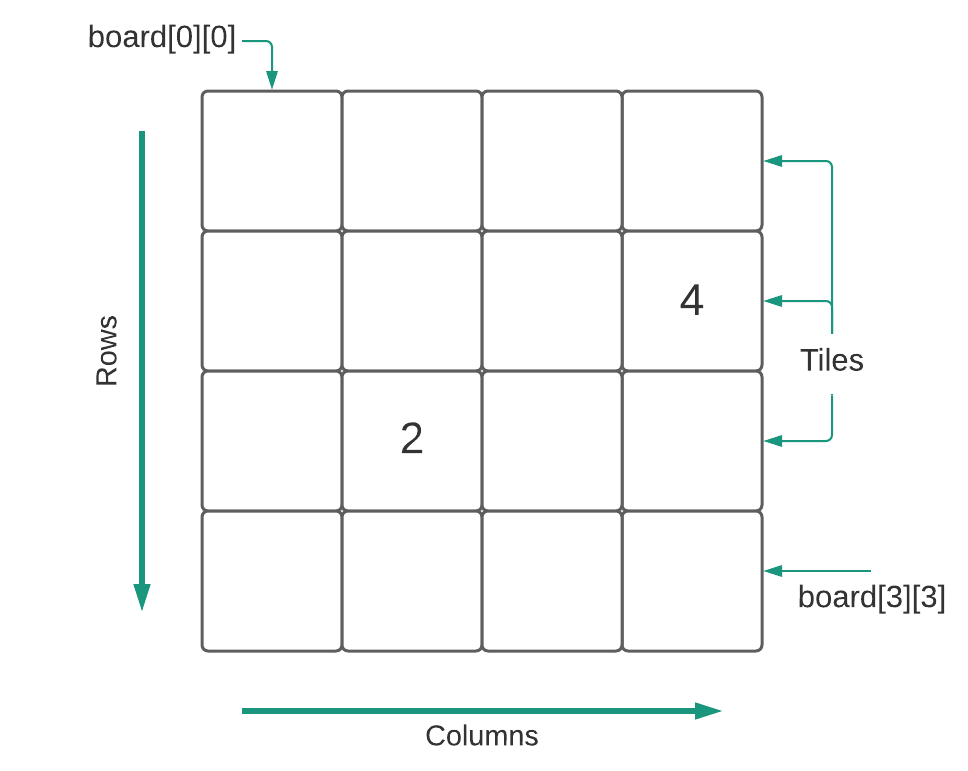
\includegraphics[scale=0.7]{board.png}
\end{center}
\newpage
\section{Overview of the design}

\indent This design applies the Module View Specification (MVC) and the Singleton design patterns. The MVC design pattern separates the computational elements from input and output elements. For this design, the MVC components are GameT (model module), Display (view module), and Controller (controller module). The model GameT module encapsulates the system's data as well as the operations on the data – storing the state of the game board and the status of the game. The view Display module displays the data from the GameT component – displaying the state of the game board and the status of the game using ASCII-based graphics. The controller module separately handles the input actions and calls the appropriate access routines of the model and view modules. Due to the MVC design pattern implementation, this design provides ease of modification.\\

The Singleton design pattern was implemented for the Display and Controller modules where there is only one instance - the getInstance() method is used to obtain the abstract object for each. \\

An UML diagram is provided below for visualizing this software architecture.\\
\begin{center}
    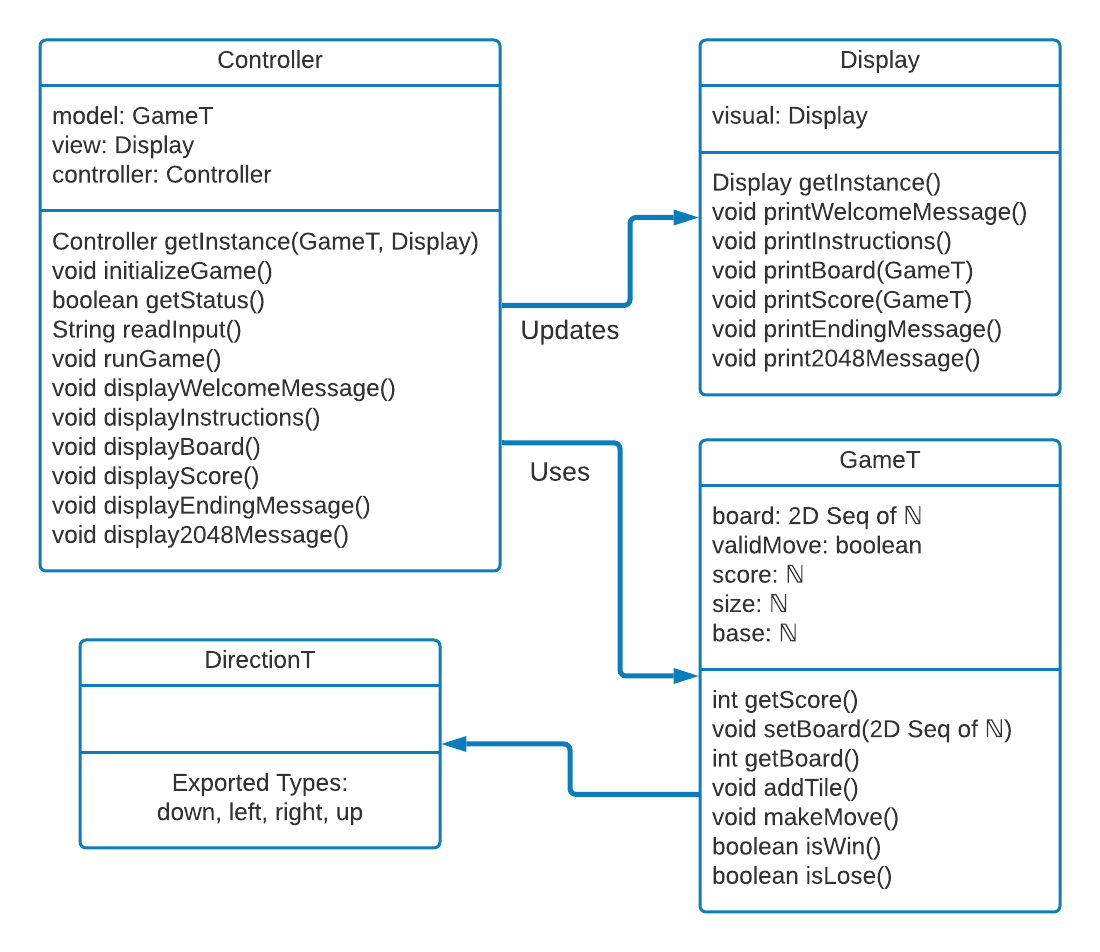
\includegraphics[scale=0.65]{UML.png}
\end{center}

\newpage

\subsection*{Likely Changes my design considers:}

\begin{itemize}
  \item My design considered likely changes regarding the data structure that is used for storing the game board. You can use a nested Array, nested ArrayList, or any other data structure that can form a 2D matrix.
  \item My design also considered that it is likely for the board size to change. You can effortlessly change the size of the matrix storing the board by altering the ``Size’’ exported constant. The access routines all consider the ``Size’’ variable when iterating through the tiles of the board. You can change the board from the default 4 by 4 to 5 by 5, 6 by 6, etc.
  \begin{itemize}
    \item This change is also considered when adding a new random tile into the board – as the size of the current board is taken into consideration. 
    \item This change is also considered within the Display module. The printBoard() access routine considers the board’s current size when displaying the content to the terminal. Although it may not look as good for large boards, it will still work.
  \end{itemize}
  \item My Display module also considers different flows of the game and as such provides different messages to be displayed.
  \item My design also considers that the controller may take in inputs of various kinds. As such, it provides a standardized input for the makeMove() access routine within the GameT module. No matter what input is provided to the controller, the controller can call the makeMove() access routine with the respective DirectionT object.
  \item My design considers that the game may be played with a base of 3 rather than 2, or any other style of gameplay. As such the ``Base’’ constant can be changed to implement many types of gameplay (base of N) – additionally, this constant changes what random tiles are added while the game will still be considered ``won’’ if a tile is greater than 2048. This change is also anticipated within the Display module by providing a general end-game message rather than a specific message for 2048.
  \item It is also considered that the gameplay may differ in regards to how many or when new tiles are added to the board. As such, the addTile() access routine is left to be manually used by a controller rather than automatically adding new tiles to the board after every move.
\end{itemize}


\newpage

\section* {DirectionT Module}

\subsection*{Module}

DirectionT

\subsection* {Uses}

None

\subsection* {Syntax}

\subsubsection* {Exported Constants}

None

\subsubsection* {Exported Types}

DirectionT = \{\\
    up, \textit{\#Moving the game tiles upward.}\\
    down, \textit{\#Moving the game tiles downward.}\\
    left, \textit{\#Moving the game tiles to the left.}\\
    right, \textit{\#Moving the game tiles to the right.}\\
\}

\subsubsection* {Exported Access Programs}

None

\subsection* {Semantics}

\subsubsection* {State Variables}

None

\subsubsection* {State Invariant}

None

\subsubsection* {Considerations}

When implemented in Java, use enums.

\newpage

\section* {GameT ADT Module}

\subsection*{Template Module}

GameT

\subsection* {Uses}

DirectionT

\subsection* {Syntax}

\subsubsection* {Exported Constants}

Size = 4  // Size of the board in each direction
Base = 2  // Base tile value

\subsubsection* {Exported Types}

None

\subsubsection* {Exported Access Programs}

\begin{tabular}{| l | l | l | p{5cm} |}
  \hline
  \textbf{Routine name} & \textbf{In} & \textbf{Out} & \textbf{Exceptions}\\
  \hline
  new GameT & & GameT & \\
  \hline
  makeMove & DirectionT &  & ~\\
  \hline
  addTile &  &  & ~\\
  \hline
  getScore &  & $\mathbb{N}$ & ~\\
  \hline
  setBoard & seq [Size,Size] of $\mathbb{N}$ &  & ~\\
  \hline
  getBoard &  & seq [Size,Size] of $\mathbb{N}$ & ~\\
  \hline
  isWin &  & $\mathbb{B}$ & ~\\
  \hline
  isLose &  & $\mathbb{B}$ & ~\\
  \hline
\end{tabular}

\subsection* {Semantics}

\subsubsection* {State Variables}

$\mathit{board}$: sequence [Size,Size] of $\mathbb{N}$\\
$score$: $\mathbb{N}$\\
$\mathit{validMove}$: $\mathbb{B}$ // Previous move was valid iff it altered the board.

\subsubsection* {State Invariant}

None

\subsubsection* {Assumptions}

It is assumed that the order of sequences within the board are be maintained. Also that when items in a sequence are traversed, they are traversed in order from start to end. It is assumed that the GameT constructor is ran before any other access routine is called. It is assumed that a random tile is added manually after every valid move - this process is not automatic within this module. setBoard() will be used only for testing purposes and will not be a part of the actual game play - as such, it is assumed that correct input will be provided by the developer.

\subsubsection* {Access Routine Semantics}

\noindent new GameT():
\begin{itemize}
\item transition: // Initiates the board to a [size][size] matrix of zeros.\\

  $\mathit{score}, validMove, board := 0, true,
  \langle \begin{array}{c}
  \langle \mbox{0}, \mbox{0}, \mbox{0}, \mbox{0} \rangle\\
    \langle \mbox{0}, \mbox{0}, \mbox{0}, \mbox{0} \rangle\\
    \langle \mbox{0}, \mbox{0}, \mbox{0}, \mbox{0} \rangle\\
    \langle \mbox{0}, \mbox{0}, \mbox{0}, \mbox{0} \rangle\\
  \end{array} \rangle
  $\\
  $\text{addTile(), addTile()  // Initial 2 random tiles}$\\

\item output: $out := \mbox{self}$
\item exception: none
\end{itemize}

\noindent getScore():
\begin{itemize}
\item output: $out := \mathit{score}$
\item exception: none
\end{itemize}

\noindent setBoard(b):
\begin{itemize}
\item transition: $board:=b$
\item exception: It is assumed that the developer testing will provide correct input. This functionality is meant only for testing purposes.
\end{itemize}
\newpage
\noindent getBoard():
\begin{itemize}
\item output: $out := \mathit{board}$
\item exception: none
\end{itemize}

\noindent addTile(): // Changes a random 0 from the board to a 2 or 4.
\begin{itemize}
\item transition: $(validMove)\Rightarrow(board[i][j]:=val)$\\
$$\text{such that }(val=\langle Base,Base*2\rangle[random(0,1)])\,\land\,(i,j:=random(0,size-1),random(0,size-1))$$
\item exception: none
\end{itemize}

\noindent makeMove($\mathit{move}$):
\begin{itemize}
\item transition: $validMove := false$\\
$$(move = up \Rightarrow board := \text{transpose}(\langle row:\text{seq of }\mathbb{N}\,|\,row\in b: \text{combine\_seq\_left}(row)\rangle)$$
$$\text{such that }b=transpose(board))$$
$$(move = down \Rightarrow board := \text{transpose}(\langle row:\text{seq of }\mathbb{N}\,|\,row\in b: \text{combine\_seq\_right}(row)\rangle)$$
$$\text{such that }b=transpose(board))$$
$$(move = left \Rightarrow board := (\langle row:\text{seq of }\mathbb{N}\,|\,row\in b: \text{combine\_seq\_left}(row)\rangle$$
$$(move = right \Rightarrow board := (\langle row:\text{seq of }\mathbb{N}\,|\,row\in b: \text{combine\_seq\_right}(row)\rangle$$
\item exception: none
\end{itemize}

\noindent isWin():
\begin{itemize}
\item out: $(\exists\,i,j:\mathbb{N}\,|\,i,j\in[0..\text{Size}-1]\land((b[i][j]\ge 2048)))$
\item exception: none
\end{itemize}

\noindent isLose(): // Checks if any move could alter a copy of the board.
\begin{itemize}
\item out: $(board=result.getBoard())$

such that result.makeMove(up), result.makeMove(down),\\ result.makeMove(left), result.makeMove(right)

such that $result : GameT \wedge result.setBoard(board)$

\item exception: none
\end{itemize}

\subsection*{Local Functions}

\noindent 
Note Pertaining To Local Functions: The order of sequences should be maintained. Items in a sequence should be traversed in order.\\

\noindent // Combines non-zero equal adjacent elements and shifts them to the left of the sequence.\\
\noindent $\mbox{combine\_seq\_left}: \text{seq of } \mathbb{N} \rightarrow \text{seq of } \mathbb{N}$\\
\noindent 
$\mbox{combine\_seq\_left}(seq) \equiv \text{shift\_seq\_left}(adj)$\\
\indent such that $(k:\mathbb{N}\,|\,k \in [0..\text{Size}-2] : (adj[k]=adj[k+1]\implies adj[k]=adj[k]*2,\\ \indent adj[k+1]=0,score:=score+adj[k]*2)$\\
\indent such that $adj := \text{shift\_seq\_left}(seq)$

$$transition: (seq \neq \text{combine\_seq\_left}(seq))\implies \, validMove:=true$$\\

\noindent // Combines non-zero equal adjacent elements and shifts them to the right of the sequence.\\
\noindent $\mbox{combine\_seq\_right}: \text{seq of } \mathbb{N} \rightarrow \text{seq of } \mathbb{N}$\\
\noindent 
$\mbox{combine\_seq\_right}(seq) \equiv \text{shift\_seq\_right}(adj)$\\
\indent such that $(k:\mathbb{N}\,|\,k \in [1..\text{Size}-1] : (adj[k]=adj[k-1]\implies adj[k]=adj[k]*2,\\ \indent adj[k-1]=0,score:=score+adj[k]*2)$\\
\indent such that $adj := \text{shift\_seq\_right}(seq)$

$$transition: (seq \neq \text{combine\_seq\_right}(seq))\implies \, validMove:=true$$\\

\noindent // Shifts non-zero elements to the left of the sequence.\\
\noindent $\mbox{shift\_seq\_left}: \text{seq of } \mathbb{N} \rightarrow \text{seq of } \mathbb{N}$\\
\noindent 
$\mbox{shift\_seq\_left}(seq) \equiv \langle i:\mathbb{N}\,|\,i \in seq \wedge i \neq 0: i\rangle || \langle j:\mathbb{N}\,|\,j \in seq \wedge j = 0: j\rangle$\\

\noindent // Shifts non-zero elements to the right of the sequence.\\
\noindent $\mbox{shift\_seq\_right}: \text{seq of } \mathbb{N} \rightarrow \text{seq of } \mathbb{N}$\\
\noindent 
$\mbox{shift\_seq\_right}(seq) \equiv \langle i:\mathbb{N}\,|\,i \in seq \wedge i = 0: i\rangle || \langle j:\mathbb{N}\,|\,j \in seq \wedge j \neq 0: j\rangle$\\

\noindent // Interchanges the rows and columns of the 2D array.\\
\noindent $\mbox{transpose}: \text{seq of (seq of }\mathbb{N})  \rightarrow \text{seq of (seq of }\mathbb{N})$\\
\noindent
$\mbox{transpose}(b) \equiv \langle i:\mathbb{N}|i\in[0..\text{Size}-1]:\langle j:\mathbb{N}|j\in[0..\text{Size}-1]:b[j][i] \rangle \rangle$\\

\noindent $\mbox{random}: \mathbb{N}\times\mathbb{N} \rightarrow \mathbb{N}$\\
\noindent
$\mbox{random}(a,b) \equiv \text{random natural number between a and b (inclusive)}$

\newpage

\section* {Display Module}

Display

\subsection* {Uses}

None

\subsection* {Syntax}

\subsubsection* {Exported Constants}

None

\subsubsection* {Exported Types}

None

\subsubsection* {Exported Access Programs}

\begin{tabular}{| l | l | l | p{5cm} |}
  \hline
  \textbf{Routine name} & \textbf{In} & \textbf{Out} & \textbf{Exceptions}\\
  \hline
  getInstance &  & Display & ~\\
  \hline
  printWelcomeMessage &  &  & ~\\
  \hline
  printInstructions &  &  & ~\\
  \hline
  printBoard & GameT &  & ~\\
  \hline
  printScore & GameT &  & ~\\
  \hline
  printEndingMessage &  &  & ~\\
  \hline
  print2048Message &  &  & ~\\
  \hline
  
\end{tabular}


\subsection* {Semantics}

\subsubsection* {Environment Variables}
window: Portion of the computer screen allocated to display the game board and messages.

\subsubsection* {State Variables}

visual: Display

\subsubsection* {State Invariant}

none

\subsubsection* {Assumptions}

The Display constructor is called for each object instance before any other access routines are called for the object. The constructor can only be called once.

\subsubsection* {Access Routine Semantics}

\noindent getInstance():
\begin{itemize}
\item transition: $\text{visual}:=(\text{visual}=\text{null}\Rightarrow\text{new Display()}) $
\item output: self
\item exception: none
\end{itemize}

\noindent printWelcomeMessage():
\begin{itemize}
\item transition: window := Displays a welcome message when user starts the game.
\item exception: none
\end{itemize}

\noindent printInstructions():
\begin{itemize}
\item transition: window := Displays the instructions on how to play the game. Possible moves, how to win, when you lose.
\item exception: none
\end{itemize}

\noindent printBoard(model):
\begin{itemize}
\item transition: window := Draws the game board onto the screen. The board is retrieved using the GameT functionality $game.getBoard()$ and the tiles are individually printed to form a 4 by 4 board. Zeros are replaced by ``O'' to improve the look of the display. The board is displayed in such a way that the top left tile is board[0][0] and the bottom right tile is board[3][3]. Space is left between the tiles to make the board easy to visually scan.
\item exception: none
\end{itemize}

\noindent printScore(model):
\begin{itemize}
\item transition: window := Displays the score of the GameT object using the $game.getScore()$ functionality.
\item exception: none
\end{itemize}
\newpage
\noindent printEndingMessage():
\begin{itemize}
\item transition: window := Displays an ending ``Game Over'' message.
\item exception: none
\end{itemize}

\noindent print2048Message():
\begin{itemize}
\item transition: window := Displays a message congratulating the player on reaching the 2048 tile.
\item exception: none
\end{itemize}

\subsubsection* {Local Functions}
\noindent Display: void $\rightarrow$ Display\\
Display() $\equiv$ new Display()

\newpage

\section* {Controller Module}

Controller

\subsection* {Uses}

GameT, Display

\subsection* {Syntax}

\subsubsection* {Exported Constants}

None

\subsubsection* {Exported Types}

None

\subsubsection* {Exported Access Programs}

\begin{tabular}{| l | l | l | p{5cm} |}
  \hline
  \textbf{Routine name} & \textbf{In} & \textbf{Out} & \textbf{Exceptions}\\
  \hline
  getInstance & GameT, Display & Controller & ~\\
  \hline
  initializeGame &  &  & ~\\
  \hline
  getStatus &  & $\mathbb{B}$ & ~\\
  \hline
  readInput &  & String & ~\\
  \hline
  runGame &  &  & ~\\
  \hline
  displayWelcomeMessage &  &  & ~\\
  \hline
  displayInstructions &  &  & ~\\
  \hline
  displayBoard &  &  & ~\\
  \hline
  displayScore &  &  & ~\\
  \hline
  displayEndingMessage &  &  & ~\\
  \hline
  display2048Message &  &  & ~\\
  \hline
  
\end{tabular}


\subsection* {Semantics}

\subsubsection* {Environment Variables}
keyboard: Scanner(System.in) // Reading input from keyboard

\subsubsection* {State Variables}

model: GameT\\
view: Display\\
controller: Controller

\subsubsection* {State Invariant}

none

\subsubsection* {Assumptions}

It is assumed that the Controller constructor is called for the object instance before any other access routines are called for the object. The constructor can only be called once. Also assuming that model and view instances are already initialized before calling the Controller constructor. 

\subsubsection* {Access Routine Semantics}

\noindent getInstance(model, view):
\begin{itemize}
\item transition: $\text{controller}:=(\text{controller}=\text{null}\Rightarrow\text{new Controller(model, view)}) $
\item output: self
\item exception: none
\end{itemize}

\noindent initializeGame():
\begin{itemize}
\item transition: model := new GameT()
\item exception: none
\end{itemize}

\noindent getStatus():
\begin{itemize}
\item transition: None
\item output: out := (model.isLose())
\item exception: none
\end{itemize}
\newpage
\noindent readInput():
\begin{itemize}
\item output: input : A String entered fromthe keyboard.
\item exception: none
\end{itemize}

\noindent runGame():
\begin{itemize}
\item transition: Operational method for running the game. The game will start with the welcome message and provide the instructions on how the game can be played. The board will be displayed and displayed again after every move. If a valid move is made, a tile is added to the board. The game will automatically end and display the ending message if no moves can be made, or it will display a congratulatory message for reaching 2048 and continue.
\item exception: none
\end{itemize}

\noindent displayWelcomeMessage():
\begin{itemize}
\item transition: view := view.printWelcomeMessage()
\item exception: none
\end{itemize}

\noindent displayInstructions():
\begin{itemize}
\item transition: view := view.printInstructions()
\item exception: none
\end{itemize}

\noindent displayBoard():
\begin{itemize}
\item transition: view := view.printBoard()
\item exception: none
\end{itemize}

\noindent displayScore():
\begin{itemize}
\item transition: view := view.printScore()
\item exception: none
\end{itemize}

\noindent display2048Message():
\begin{itemize}
\item transition: view := view.print2048Message()
\item exception: none
\end{itemize}


\subsection*{Local Functions}

\noindent
\noindent $\mbox{Controller}: \text{GameT} \times \text{Display} \rightarrow \text{Controller}$\\
\noindent 
$\mbox{Controller}(model,view) \equiv \text{new Controller}(model,view)$\\

\newpage

\section*{Critique of Design}

\begin{itemize}
    \item I chose to specify the GameT module an as ADT rather than an abstract object. This is because it is more convenient to create a new instance of the board after a user chooses to start a new game.
    \item The Controller and Display modules are specified as single abstract objects as these modules are shared resources and only one instance is required to control the actions during runtime. This way, conflicts and unexpected state changes can be avoided.
    \item The setBoard() method was included strictly for testing purposes – it is therefore largely assumed that the developer using it will provide correct inputs and would use it to test other modules rather than test the method itself.
    \item Consistency can be expressed by maintaining a consistent pattern to how access routines and variables are named. It can also be expressed by how such things are ordered – including the parameters to the access routines. My design puts a strong emphasis on consistency in order to make the MIS easy to follow:
    \begin{itemize}
        \item Whenever the directions or direction-based conditions are listed, I made sure to always keep the order the same: up, down, left, right. This is also true for the DirectionT module.
        \item The simple setters and getters of a module are grouped together and outlined first.
        \item A 2D matrix input is always referred to as “b” to provide intuition about what the input is since the game matrix itself is called “board”.
        \item Whenever a GameT input is needed or referred to, it is called “model”. Whenever a Display object is referred to, it is called “view”. Furthermore, the inputs for Controller are taken in the same order every time – model, view.
        \item The Display and Controller access routines share very similar names – the only difference between most is that within Controller, they have prefix “display” and in Display the prefix is “print”.
    \end{itemize}
    \item Essentiality describes how unnecessary access programs are omitted. My MIS implements essentiality as every access program is used to produce the flow of the 2048 game. Every access program is needed to make a unique move, print a message according to the state of the game, or check the status of the current game. The access routines that perform simple services are used in multiple stages and that is why they are separated – such as the shift\_seq\_left and right routines that are essential to the movement of the board. The custom congratulatory message for reaching a 2048 tile may not be essential as it can be displayed just once per game, but because it is a rare occurrence, I separated it from the rest of the design to maintain readability. It is still essential as it signifies reaching the main objective of the game – it’s simply rarely used.
    \item The goal of generality is to solve more general problems. While designing my MIS, I decided to try and make the movement of the board as general as I can. As such, I created the shift\_seq\_left and shift\_seq\_right routines. These are fairly general and do not immediately associate with the 2048 game. They simply move the non-zero elements of a sequence to the left or right. Expanding from this, I created the combine\_seq\_left and combine\_seq\_right routines. These routines combine non-zero equal adjacent elements and shift them to the left or right. The Display and Controller routines are also kept semi-general as the messages do not rely on the game state and can simply be called if needed. The messages are not strictly bounded to the GameT object’s state. Lastly, the DirectionT module was kept general using enumerated types to represent the directions that the board can move in.
    \item A minimal interface avoids access routines that offer two different services that might be requested separately by the user. I tried to keep my access routines minimal throughout the MIS – getters, setters, and printing routines can easily be kept minimal. However, certain access routines are required to provide multiple services in order to keep the MIS easy to read and implement. The following explain instances where the principle of minimality is violated.
    \begin{itemize}
        \item My GameT module violates minimality as it must initialize the board, validMove state variable, score, and must also add two random tiles to the board. 
        \item Furthermore, within the GameT combine\_seq routines, I return a sequence output and also update the validMove state variable. This makes the MIS far easier – rather than creating a new routine to update the validMove state variable. We can simply check if the routine’s actions altered the input sequence and that would tell if the move was valid. 
        \item Also within the combine\_seq routines, I must update the score respectively to what elements are being combined – I would not be able to do this outside of the routine that is doing the combining.
        \item The Controller module cannot be minimal because playing a game consists of many different things going on at once – making a move, displaying messages, and initializing new games.
    \end{itemize}
    \newpage
    \item This design implements high cohesion and low coupling. This means that the components of the module are closely related – this is expressed by the MVC design pattern that was incorporated. Low coupling is seen as the modules do not strongly depend on other modules – while they are all needed to play the game, they do not crash or break without another.
    \item Information hiding is respected within my MIS design as things that are likely to change are hidden. The exported constants that determine the gameplay (such as size and base), the state variables, and the local functions are all kept private – hidden. The implementation secrets are hidden from the user – how the movements are actually conducted. All the user has access to is what they need to play.
    \item The print access routines within the Display (view) module are not completely necessary. The Controller module has access routines that simply call for the print access routines - therefore, instead of calling them we could simply put them within the Controller module. We do not necessarily need the functionality within the Display module - it would be enough within the Controller. However, this was done to maintain organization and also reduce the dependency of the game on just the controller. This way, we can leave running the game to the Controller and modify the messages within the Display module.
    \item Comprehensive unit testing was done for the GameT module while the other modules were indirectly yet thoroughly manually tested using the controller. Unit tests were conducted on carefully selected cases to cover many complex cases as well as base cases. For example, some boards used were the empty board, one with only corner tiles, one with all filled except one spot, one completely filled, alternating empty rows and columns, etc. I tested every public GameT method for most of these cases to see how the program performs in intricate situations.
\end{itemize}
\newpage
\section*{Answers to Questions}

Q1. Draw a UML diagram for the modules in A3

\begin{center}
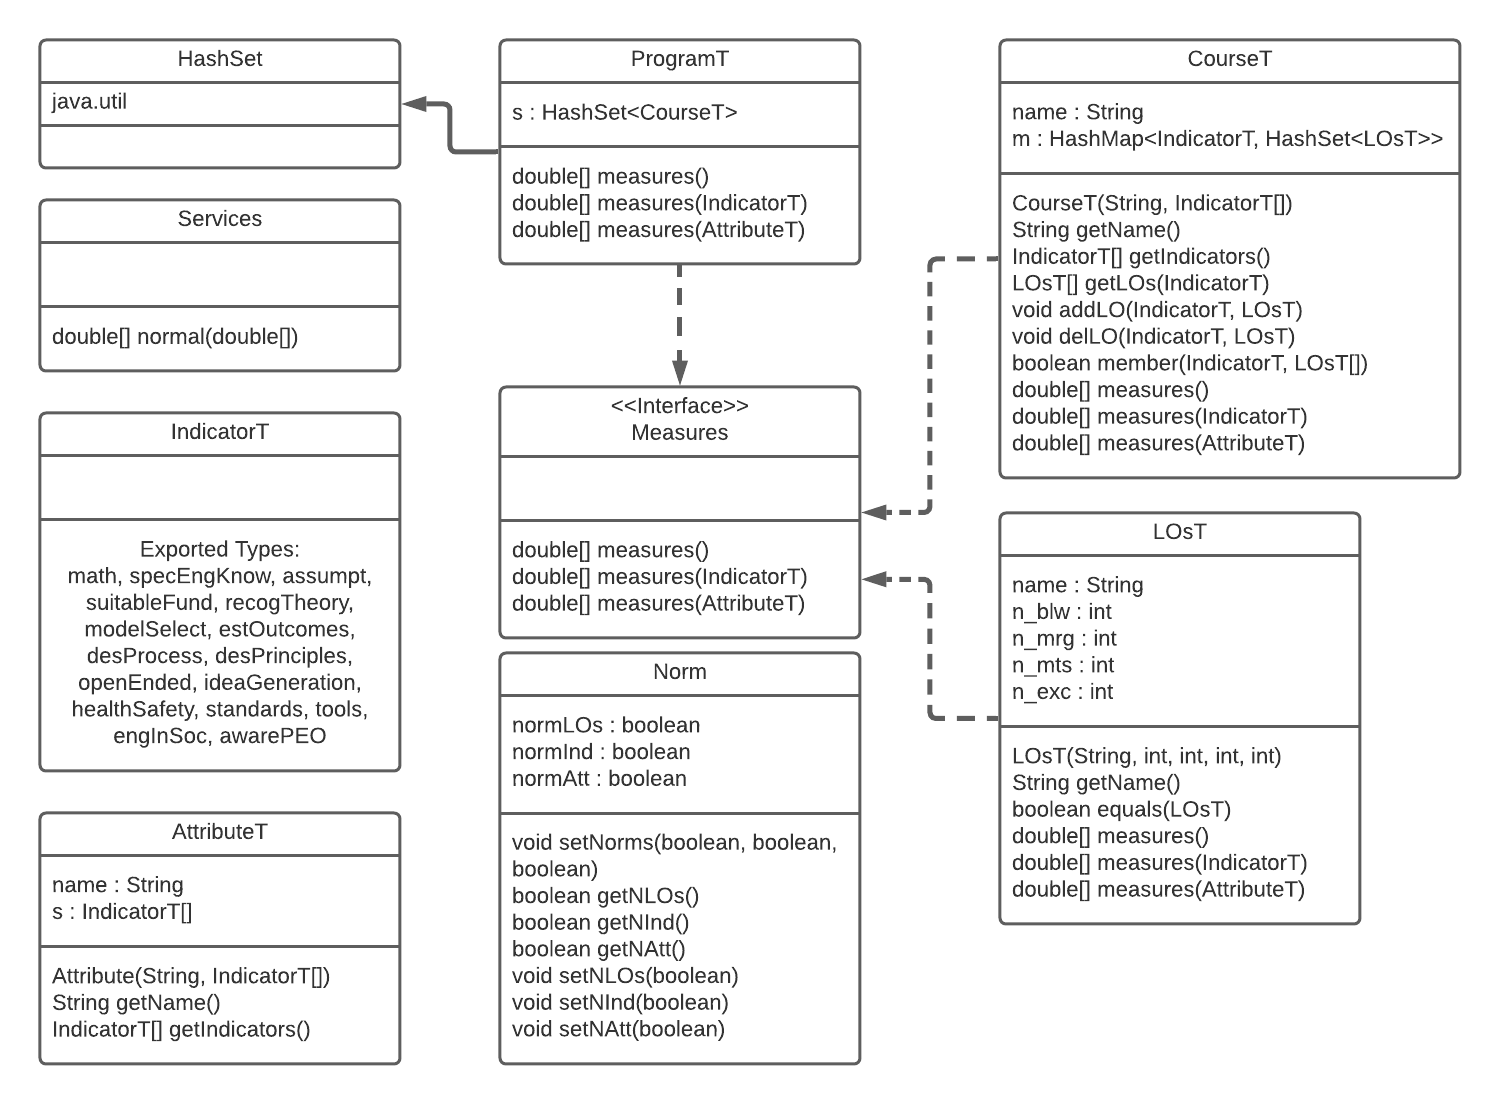
\includegraphics[scale=0.7]{Q1_UML.png}
\end{center}

\end {document}
